\documentclass[12pt, landscape]{article}

\usepackage[utf8]{inputenc}
\usepackage[T1]{fontenc}
\usepackage[a4paper, margin=0.5in]{geometry}
\usepackage{xcolor}
\usepackage{tikz}
\usepackage{enumitem}
\usepackage{setspace}
\usepackage{amssymb}
\usepackage{helvet}
\renewcommand{\familydefault}{\sfdefault}
\usetikzlibrary{positioning, shapes.geometric, arrows.meta}

% Brand colors matching the screenshot
\definecolor{myteal}{RGB}{0, 100, 100}
\definecolor{myorange}{RGB}{236, 112, 99}
\definecolor{boxblue}{RGB}{214, 234, 248}
\definecolor{boxgreen}{RGB}{213, 245, 227}
\definecolor{boxorange}{RGB}{250, 215, 161}
\definecolor{boxyellow}{RGB}{252, 243, 207}
\definecolor{boxpink}{RGB}{250, 219, 216}
\definecolor{boxcyan}{RGB}{209, 242, 235}
\definecolor{boxpurple}{RGB}{232, 218, 239}

\begin{document}
\pagestyle{empty}

% --- TITLE ---
{\noindent\LARGE\bfseries\color{myteal} Proposed System \& Architecture} \\[0.1cm]
{\color{myorange}\rule{3cm}{2.5pt}} 

\vspace{0.8cm}

\noindent
\begin{minipage}[t]{0.52\textwidth}
    {\large\bfseries\color{myteal} System Architecture} \\[0.1cm]
    \textcolor{gray!50}{\rule{\textwidth}{0.8pt}}
    
    \vspace{0.5cm}
    \centering
    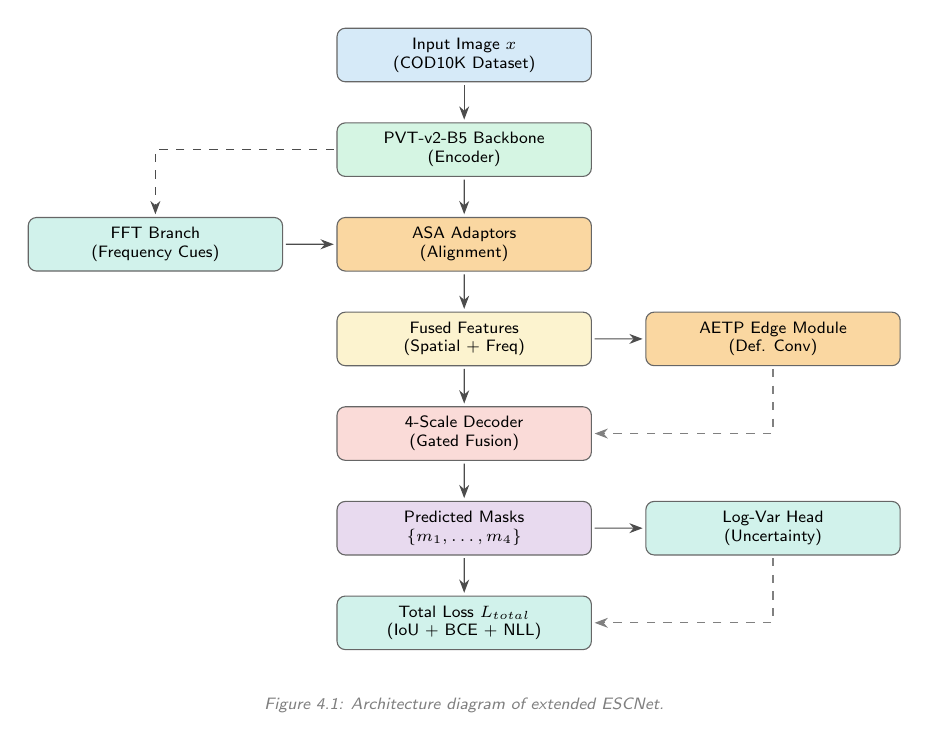
\begin{tikzpicture}[
        node distance=0.6cm and 0.5cm, 
        font=\scriptsize, 
        scale=0.85, 
        every node/.style={transform shape}
    ]

    \tikzset{
        base/.style={rectangle, rounded corners=3pt, draw=black!60, minimum width=3.8cm, minimum height=0.8cm, align=center},
        arrow/.style={->, >=Stealth, shorten >=1pt, shorten <=1pt, draw=black!70}
    }

    % Central Column
    \node[base, fill=boxblue] (input) {Input Image $x$\\(COD10K Dataset)};
    \node[base, fill=boxgreen, below=of input] (pvt) {PVT-v2-B5 Backbone\\(Encoder)};
    \node[base, fill=boxorange, below=of pvt] (asa) {ASA Adaptors\\(Alignment)};
    \node[base, fill=boxyellow, below=of asa] (fuse) {Fused Features\\(Spatial + Freq)};
    \node[base, fill=boxpink, below=of fuse] (decoder) {4-Scale Decoder\\(Gated Fusion)};
    \node[base, fill=boxpurple, below=of decoder] (mask) {Predicted Masks\\$\{m_1, \dots, m_4\}$};
    \node[base, fill=boxcyan, below=of mask] (loss) {Total Loss $L_{total}$\\(IoU + BCE + NLL)};

    % Side Branches
    \node[base, fill=boxcyan, left=0.8cm of asa] (fft) {FFT Branch\\(Frequency Cues)};
    \node[base, fill=boxorange, right=0.8cm of fuse] (edge) {AETP Edge Module\\(Def. Conv)};
    \node[base, fill=boxcyan, right=0.8cm of mask] (unc) {Log-Var Head\\(Uncertainty)};

    % Main Arrows
    \draw[arrow] (input) -- (pvt);
    \draw[arrow] (pvt) -- (asa);
    \draw[arrow] (asa) -- (fuse);
    \draw[arrow] (fuse) -- (decoder);
    \draw[arrow] (decoder) -- (mask);
    \draw[arrow] (mask) -- (loss);

    % Side Arrows
    \draw[arrow] (fft.east) -- (asa.west);
    \draw[arrow] (fuse.east) -- (edge.west);
    \draw[arrow] (mask.east) -- (unc.west);
    
    % Dashed Arrow from PVT to FFT
    \draw[arrow, dashed] (pvt.west) -| (fft.north);
    
    % Dashed auxiliary arrows
    \draw[arrow, dashed, draw=gray] (edge.south) |- (decoder.east);
    \draw[arrow, dashed, draw=gray] (unc.south) |- (loss.east);

    \node[below=0.6cm of loss, font=\scriptsize\itshape, text=gray] {Figure 4.1: Architecture diagram of extended ESCNet.};

    \end{tikzpicture}
\end{minipage}
\hfill
\begin{minipage}[t]{0.45\textwidth}
    {\large\bfseries\color{myteal} Working of the Pipeline} \\[0.1cm]
    \textcolor{gray!50}{\rule{\textwidth}{0.8pt}}
    
    \begin{enumerate}[label=\textcolor{myorange}{\arabic*.}, leftmargin=*, nosep, itemsep=6pt]
        \item \textbf{Input Image ($256 \times 256$)} feeds into the \textbf{PVT-v2-B5 backbone} to extract global context.
        \item \textbf{FFT Branch} injects frequency-domain texture information to refine boundary ambiguities.
        \item \textbf{ASA Adaptors} map multi-scale features to a uniform 128-channel space.
        \item \textbf{AETP Module} applies deformable convolution to extract sharp edge priors.
        \item \textbf{Gated Decoder} fuses the features level-by-level to recover the segmentation mask.
        \item \textbf{Log-Var Head} outputs per-pixel aleatoric uncertainty ($\log \sigma^2$).
    \end{enumerate}

    \vspace{0.8cm}

    {\large\bfseries\color{myteal} Tools \& Libraries} \\[0.1cm]
    \textcolor{gray!50}{\rule{\textwidth}{0.8pt}}
    \begin{itemize}[label=\textcolor{myorange}{\tiny$\blacksquare$}, leftmargin=*, nosep, itemsep=4pt]
        \item \textbf{Language}: Python 3.11, \textbf{Framework}: PyTorch 2.3
        \item \textbf{Backbone}: PVT-v2-B5 (Pretrained on ImageNet-22K)
        \item \textbf{Hardware}: Apple Silicon (MPS Backend)
        \item \textbf{Dashboard}: Flask REST API + Vanilla HTML/JS
        \item \textbf{Loss Weights}: Adaptive NLL optimization
    \end{itemize}
\end{minipage}

\end{document}
